\chapter{Introduction}

% Explain what I am doing and why to my Mum...
% Outline of Chapters
	% One sentence per chapter
% Contributions
% 	Evaluate current state of the art
% 	Testing environment setup (eg github)
% 	Design and implement superior algo

The DNA sequence of an organism encodes the information necessary for its
survival and reproduction.
Because of its key role in living organisms, DNA sequencing has become a
burgeoning field in both academic research and clinical medicine.
%Knowledge of this sequence can be used to identify,
%diagnose and treat genetic diseases.
Nanopore sequencing is one such approach used to determine the order of
DNA nucleobases (A, C, T and G) in a molecule.

Nanopore sequencing records the ionic current as a DNA molecule passes through a
nanoscale protein pore (or \textit{nanopore}).
This process is depicted in Figure \ref{fig:dna-nano}.
Disturbances in the ionic current
signal are used by computational algorithms to determine the DNA sequence.
Oxford Nanopore Technologies (ONT) is the leading producer of nanopore
sequencing machines -- such as the portable MinION shown in Figure \ref{fig:minion}.

%\begin{wrapfigure}{r}{0.5\textwidth}
\begin{figure}
\centering
\includegraphics[width=0.48\textwidth]{plots/minion.png}
\caption{\label{fig:minion}The MinION is a highly portable nanopore sequencing
device manufactured by ONT which weighs only 450g.}
%\end{wrapfigure}
\end{figure}

%\begin{wrapfigure}{r}{0.5\textwidth}
\begin{figure}
\centering
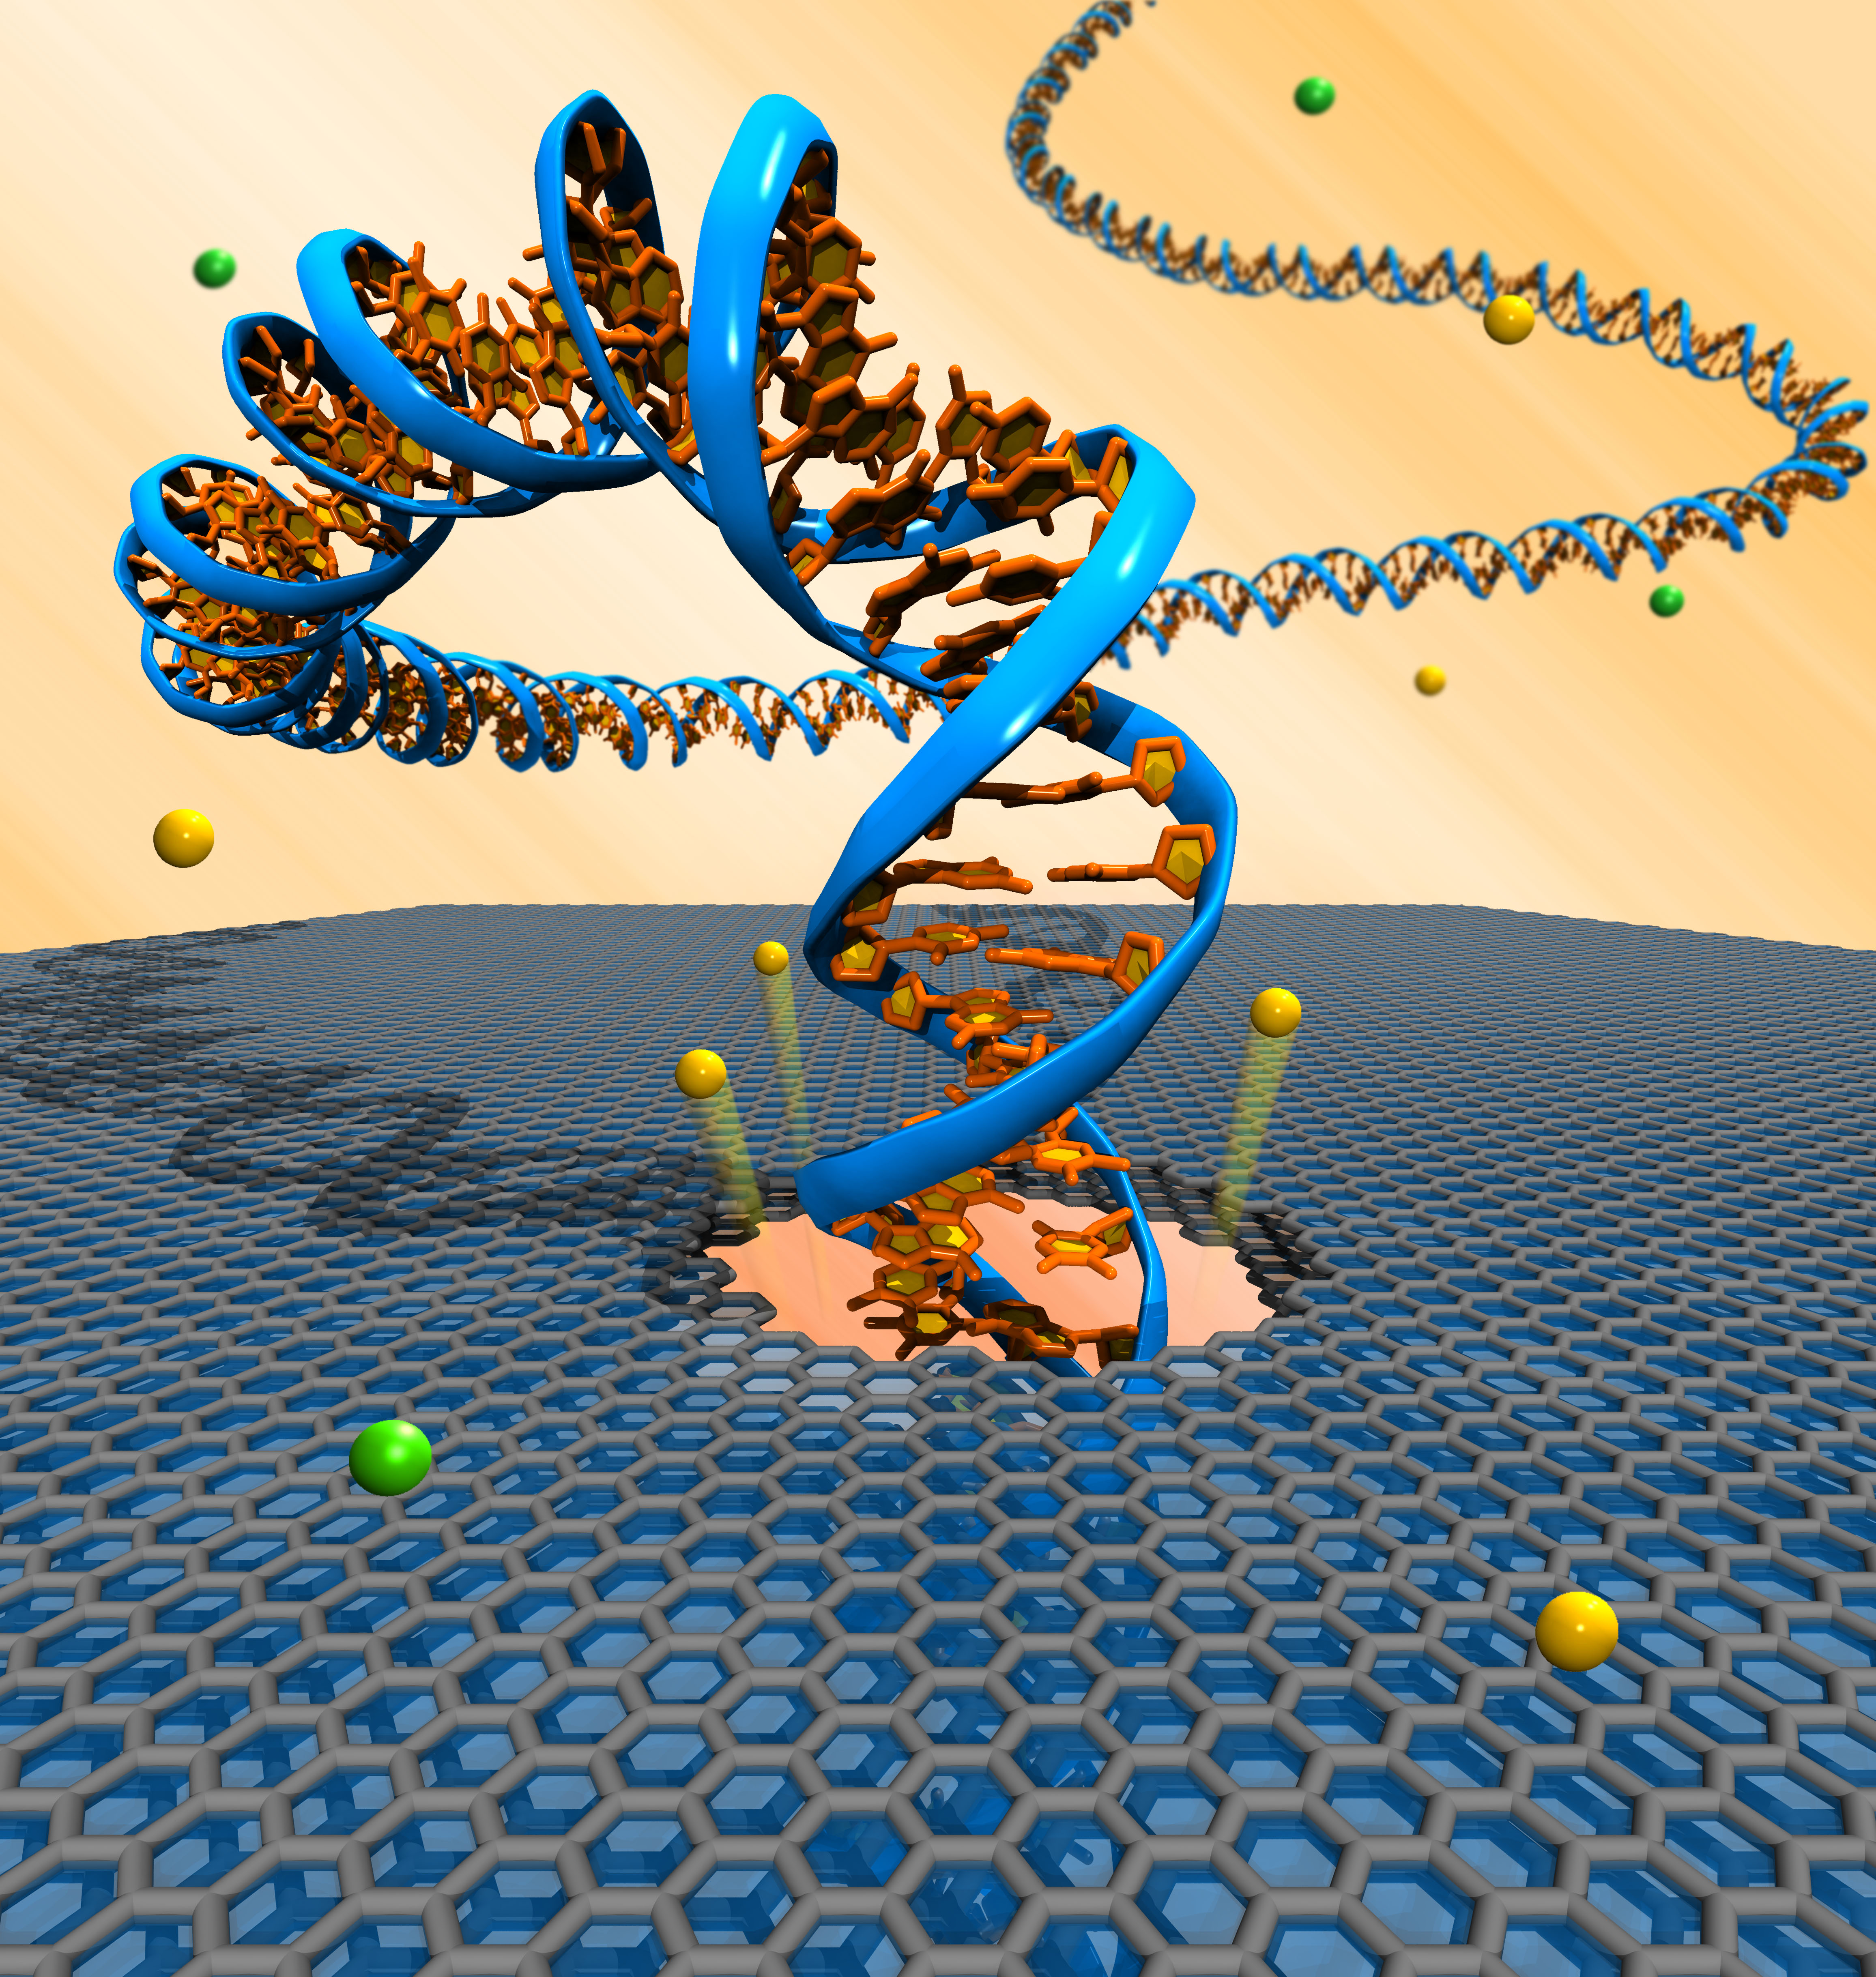
\includegraphics[width=0.48\textwidth]{plots/dna-nano.png}
\caption{\label{fig:dna-nano}A DNA molecule passing through a nanopore in an
electrolytic solution.}
%\end{wrapfigure}
\end{figure}


The problem is that nanopore sequencing produces a huge volume of data which is
being recorded at an increasing rate and often needs to be archived for several
years due to certain data regulations.
For instance, the Genomic Technologies Group at the Garvan Institute of Medical
Research regularly perform between 5 and 10 clinical human DNA sequencing runs a
week which need to be archived for up to 10 years.
This amounts to between 260 and 520 terabytes of new data each year, which costs
up to USD \$6000 a year to archive using Google Cloud Storage. Over 10 years,
this amount of data would accumulate to almost 28 petabytes or roughly USD
\$\num{330000} in storage costs.

Data compression solves this problem by identifying and removing statistical
redundancies in the data and hence decreasing its overall size.
Compression methods which achieves this without losing any information are
known as \textit{lossless}. These methods can then be reversed to decompress the
compressed data and reobtain the original information. One such lossless
compression method, known as entropy encoding, attempts to approach the entropy
of the data -- the level of uncertainty inherent in the data's distribution --
by replacing each symbol with a binary code. Huffman coding is a famous example
of entropy encoding which uses the probability distribution of the symbols to
construct optimal-length binary codes.

The state-of-the-art method used to compress nanopore signal data begins by
taking the differences between each successive point. These differences, or
\textit{deltas}, are then transformed to the positive integers by the zig-zag
encoding. Each zig-zag delta is recorded using the minimum number of bytes
possible in an encoding known as Stream VByte. Then, this is compressed using
zstd -- a very fast compression algorithm which combines entropy encoding with
dictionary-matching. This method reduces the data to 34.1\% of its original
size. However, it remains to discover whether more space can be saved through a
better understanding of nanopore signal data.

%It typically produces around 1 TiB of data for
%a human DNA sequencing run.
% How many runs by some well known institute or project to put into perspective?
% G42 (60 promethions 50 samples a week per prom = 3000 samples), Nottingham, UCSC, Washington
%The Genomic Technologies Group at the Garvan Institute of Medical Research
%regularly perform 5-10 clinical human DNA sequencing runs a week which need to
%be archived for up to 10 years. This amounts to between 260 and 520 TiB a year.
% How much data produced in certain years, for different projects, etc. ?
% normal research 5 years
% medical related 5-10 years
% NHMRC ARC uni data regulations

%Around 3 billion bases in the human genome.
%Each base is recorded by roughly 10 signal points (=30 billion points).
%2 bytes per integer (=60 GiB)
%To increase sequencing accuracy each base is recorded many times over. For 20 x coverage (=1 TiB)
%Many labs doing human DNA sequencing at a large rate.

\section{Contributions}

The first systematic analysis of nanopore DNA signal data architecture was
conducted including the articulation of characteristic features as relevant to
data compression. A novel measure for comparing the practical suitability of two
compression methods is proposed.

A new state-of-the-art compression method was designed which reduces the data to 33.4\%
of its original size (0.7\% better than the previous state-of-the-art). It
combines a novel encoding of the signal data's zig-zag deltas known as vbbe21
with dynamic domain-specific stall encoding and predictive range coding. Three
range coding model predictors -- order-0, order-1 and secondary symbol
estimation (SSE) -- were evaluated and found to reduce the data to 34.1\%,
33.9\% and 33.4\% of its original size respectively.
An alternative static Huffman compression method is proposed which also
outperforms the state-of-the-art in terms of space reduction, reducing the data
to 33.9\% of its original size.

The first detailed and comprehensive benchmark of nanopore signal data
compression, including both existing and novel methods, was conducted and
released for public access.

\section{Thesis Outline}

To begin with, we provide a detailed introduction to nanopore sequencing,
information theory and data compression (Chapter \ref{chap:litreview}). Then, we
explore the nature of the data through a systematic analysis which involves
identifying its characteristics and understanding its relevant transformations
(Chapter \ref{chap:data}).

Next, the problem space is defined with respect to the requirements of
practicing bioinformaticians and a mathematical metric for comparing the
suitability of two compression methods is presented (Chapter
\ref{chap:probspace}). Afterwards, several novel encodings and compression
methods for nanopore signal data are proposed and detailed, including the
evaluation of their running times and space savings (Chapter
\ref{chap:methodology}).

The results of a comprehensive benchmark of the existing and novel methods are
then contextualised, presented and visualised (Chapter \ref{chap:results}).
Following this is a detailed discussion of the results including their impact
and limitations, as well as an overview of future work in the landscape of
nanopore signal compression (Chapter \ref{chap:disc}). Finally, we conclude by
summarising the crucial findings of this thesis (Chapter \ref{chap:conclusion}).
